% !TeX program = xelatex
\documentclass[UTF8,a4paper,12pt]{ctexart}

% 所有宏包和统一排版设置集中在这里。
% 本文件只保存全局宏包和排版设置，通常不需要频繁修改。

\usepackage[margin=2.5cm]{geometry}
\usepackage{amsmath}
\usepackage{amssymb}
\usepackage{booktabs}
\usepackage{graphicx}
\usepackage{makecell}
\usepackage{multirow}
\usepackage{needspace}
\usepackage{tabularx}
\usepackage[hidelinks]{hyperref}

% 图片统一放在 figures/ 目录；插图时可以只写文件名。
\graphicspath{{figures/}}


\title{FlexPPI：基于几何 Transformer 的逐残基柔性预测\\及其在 TCR--pMHC 复合物上的伙伴上下文诊断}
\author{}
\date{}

\begin{document}

\maketitle

\begin{abstract}
从单个静态结构快速估计蛋白质的残基级柔性，有望补充分子动力学模拟在计算成本
和数据覆盖上的不足；然而，静态结构模型能否利用结合伙伴信息并正确恢复界面
动力学，仍缺少严格的外部检验。本文提出 FlexPPI，一种基于主链局部框架和不变点
注意力、对整体旋转和平移保持不变的几何 Transformer，可从静态单链或多链结构
预测逐残基均方根波动（RMSF）、侧链构象熵 $H_\chi$、溶剂可及表面积（SASA）
及其不确定性。模型在 ATLAS 与 DynaRepo 轨迹标签上训练，在 ITrace
TCR--pMHC 复合体上进行外部评估。排除精确训练 PDB 重叠后，完整复合物在 244 个
复合体上的平均 RMSF Spearman 为 0.740；在保留结合态坐标不变、只删除对侧伙伴的
受控消融中，删伙伴子复合物为 0.691。完整输入将绝对 MAE 从
$0.373\,\text{\AA}$ 降至 $0.346\,\text{\AA}$，同时在直接接触区产生集中但近乎
单向的负向 RMSF、$H_\chi$ 和 SASA 修正。该结果证明模型利用了伙伴几何，却不等同
于真实 apo/holo 动力学变化，并揭示了静态几何模型把接触过度概括为局部受限的边界。
\end{abstract}

% 正文按章节拆分。平时主要编辑 sections/ 目录中的文件。
% !TeX root = ../paper.tex

\section{引言}

蛋白质功能由结构与构象运动共同决定。实验结构和结构预测模型通常给出单个或少量
构象，而真实蛋白质在热涨落下持续采样构象集合；界面形成还会重新分配局部运动，
使部分残基受限，并可能在界面外产生协同或补偿性变化。分子动力学（molecular
dynamics，MD）能够在原子分辨率下刻画这些过程，但其计算成本限制了大规模应用。
ATLAS 和 DynaRepo 等标准化轨迹资源缓解了动态数据分散、模拟协议不一致和重复不足
的问题\cite{vandermeersche2024atlas,mokhtari2026dynarepo}，同时也使“由一个静态
结构预测残基级动态量”成为可监督学习任务。本文关注三个互补描述符：均方根波动
（root mean square fluctuation，RMSF）度量主链位置涨落，侧链构象熵
$H_\chi$ 描述旋转异构状态的多样性，溶剂可及表面积（solvent-accessible surface
area，SASA）反映局部溶剂暴露。三者均可由轨迹估计，但分别对应不同层面的动态
信息，不能相互替代。

从静态结构预测柔性的既有方法大体分为物理近似、结构统计和数据驱动模型。正则模态
与粗粒化模拟以较低成本近似集体运动；FastProtFlex 使用原子邻接图的局部拓扑统计
预测相对 RMSF\cite{praznikar2026fast}，ProDy 提供基于 C$\alpha$ 接触网络的
ANM/GNM 模态分析\cite{zhang2021prody}；RMSF-net 将 PDB 或 cryo-EM 密度体素化后
用三维卷积网络预测柔性\cite{song2024rmsfnet}；Flexpert 与 BackFlip 分别以
序列--结构表示和等变主链网络学习残基级柔性
\cite{kouba2025flexpert,viliuga2025backflip}。与这些直接预测器不同，AlphaFlow
通过 flow matching 生成构象集合，可从采样坐标导出 RMSF\cite{jing2024alphaflow}。
另一方面，几何深度学习通过距离、局部坐标系或等变表示消除任意全局坐标系的影响。
SE(3)-Transformer 将旋转和平移对称性纳入注意力计算\cite{fuchs2020se3}，
AlphaFold2 的不变点注意力（invariant point attention，IPA）利用局部框架和三维
查询点更新残基表示\cite{jumper2021alphafold}；
PeSTo 与 DeepInteract 进一步表明，几何注意力能够直接建模蛋白质界面及伙伴特异的
残基关系\cite{krapp2023pesto,morehead2022deepinteract}。这些进展说明静态结构中
包含可学习的柔性和界面线索，但并不自动保证模型能够恢复结合伙伴所对应的动力学
变化。

现有评估通常把一个蛋白质内部的预测 RMSF 与参考 RMSF 相关联。该指标适合衡量
“哪些残基相对更柔”，却不能回答两个与蛋白质结合直接相关的问题。第一，模型在
完整复合物上取得较高的总体相关性，可能主要来自稳定的二级结构和非界面区域，
而非对界面动力学的正确刻画。第二，将伙伴删除所造成的预测变化同时包含跨链接触、
输入长度和注意力归一化变化；如果两种输入仍共享结合态坐标，该差值只能称为模型
上下文响应，不能等同于具有独立游离态轨迹支持的 apo/holo 响应。抗体研究中对
结合前后 CDR 构象变化的分析同样强调，局部构象改变、相对框架位移和构象选择必须
分别定义\cite{liu2024cdr}。因此，柔性模型需要同时接受整体排序、界面分层、残基级
定位和受控上下文消融，而不能只报告一个汇总相关系数。

为此，本文提出 FlexPPI。模型以氨基酸类别、实验条件和主链坐标为输入，用固定
N--C$\alpha$--C 局部框架构造旋转和平移不变的残基对几何，并通过四层 IPA 在完整
多链结构中传播伙伴信息。概率状态头为每个残基预测 RMSF、$H_\chi$ 和 SASA 的均值
与方差；噪声感知目标将重复轨迹或时间窗口间方差显式并入训练。模型首先在 ATLAS
和 DynaRepo 上学习绝对状态。训练结束后，我们冻结检查点，在 ITrace 的 245 个
TCR--pMHC 复合体和 735 条轨迹上构建外部评估。主要伙伴消融保持结合态坐标不变，
仅删除对侧组分：pMHC 残基比较完整五链与 pMHC-only 输入，TCR 残基比较完整五链与
TCR$\alpha\beta$-only 输入；五条孤立链只作为进一步拆解子复合物的敏感性分析。
该设计将“静态结构能否预测 MD 真值”与“模型是否响应对侧伙伴上下文”分开检验，
并避免把 pMHC 内部或 TCR$\alpha\beta$ 内部相互作用混入主要伙伴效应。

外部结果揭示了模型能力的明确边界。排除唯一精确 PDB 重叠 3KXF 后，FlexPPI 在
244 条抗原肽内的平均残基 Spearman 为 $0.302$，能够恢复九肽 P1 活跃和 P2/P8
受限的群体趋势，但遗漏 P6 活动峰；最活跃残基命中率仅为 34.0\%。在全部链上，
完整复合物预测的平均 Spearman 为 $0.740$，高于逐链 BackFlip-seq 的 $0.704$、
FastProtFlex 的 $0.685$ 和 RMSF-net-PDB 的 $0.526$；但是，BackFlip-seq 在线性
相关和标准化误差上更好，结构版 BackFlip 在 CDR3 内也明显领先。FlexPPI 的总体
排序增益主要来自非界面区域。进一步的固定坐标伙伴消融显示，完整输入相对删伙伴
子复合物将 Spearman 从 0.691 提高到 0.740，并将绝对 MAE 从
$0.373\,\text{\AA}$ 降至 $0.346\,\text{\AA}$；但加入伙伴会近乎单向地下调接触
残基的 RMSF、$H_\chi$ 和 SASA。该偏置改善了 MHC 接触面的相对刚性，却将 MD 中
较柔的 TCR 接触面和 CDR1/2$\beta$ 错误压低。模型由此学到了可定位但过度单向的
伙伴约束，而没有充分恢复界面两侧的动力学分工。

本文的贡献包括三个方面：（1）构建一个同时预测 RMSF、侧链构象熵和 SASA 及其
不确定性的多链几何 Transformer，并给出从轨迹标签、局部框架到噪声感知目标的
完整定义；（2）在训练完成后引入具有三条独立 MD 重复的 ITrace 队列，以残基排序、
肽位置、接触分层和 TCR 链别动力学检验静态模型，而不是将 MD 描述本身作为模型
贡献；（3）通过同一检查点的固定坐标上下文消融，区分模型已被外部真值支持的能力
与仍待独立 apo/holo 轨迹验证的机制假设。本文不把 RMSF、$H_\chi$ 或 SASA 的变化
直接换算为结合自由能，也不把共享结合态坐标的删链差值解释为真实结合响应。

% !TeX root = ../paper.tex

\section{相关工作}

\subsection{蛋白质柔性数据与静态结构预测}

蛋白质柔性可由晶体 B 因子、NMR 构象集合、粗粒化模拟或全原子 MD 近似，但这些
信号对应的时间尺度、实验条件和物理含义并不相同。ATLAS 采用标准化协议和重复轨迹
覆盖结构多样的蛋白质，为跨体系比较 RMSF 提供了统一来源
\cite{vandermeersche2024atlas}；DynaRepo 将数据范围扩展到蛋白质复合物及配对的
瞬时相互作用体系，并提供更长的重复模拟\cite{mokhtari2026dynarepo}。在预测方法上，
FastProtFlex 以原子图的 graphlet degree vector 构造轻量线性模型，强调速度和局部
拓扑可解释性\cite{praznikar2026fast}；Flexpert-Seq/Flexpert-3D 借助预训练蛋白语言
模型分别从序列或序列--结构联合输入预测 RMSF\cite{kouba2025flexpert}。这些工作主要
评价单个蛋白内部的绝对柔性排序。FlexPPI 与之互补：它以多链结构为输入，同时预测
三类动态描述符，并将伙伴上下文作为需要独立审计的变量。

\subsection{几何深度学习与蛋白质界面建模}

三维蛋白质模型必须处理全局坐标系的任意性。SE(3)-Transformer 通过张量场和等变
注意力传播方向信息\cite{fuchs2020se3}；AlphaFold2 的 IPA 则在残基局部框架中生成
标量与三维点查询，并以全局点间距离构造不变注意力分数
\cite{jumper2021alphafold}。FlexPPI 采用后一条路线：主链框架在编码过程中固定，
网络输出对整体旋转和平移不变的逐残基标量，而不是更新原子坐标。

针对蛋白质相互作用，DeepInteract 通过随层演化的残基对几何预测伙伴特异的界面
接触\cite{morehead2022deepinteract}；PeSTo 直接处理原子点云，以标量--向量几何
Transformer 识别多类分子界面\cite{krapp2023pesto}；HERN 则使用残基/原子双层
等变图迭代优化抗体--抗原界面\cite{jin2022hern}。这些模型的目标分别是接触分类、
界面识别或结构生成，不能直接给出热涨落幅度。FlexPPI 研究的是另一问题：静态几何
中的伙伴信息能否预测 MD 定义的残基级柔性，以及该信息在界面两侧是否具有正确方向。

\subsection{结合前后变化与热力学边界}

结合相关变化至少包含三个不同层次：静态构象差异、构象集合或涨落的变化，以及结合
自由能。对抗体 CDR 的大规模结构比较表明，大多数非 H3 环在结合前后仅发生有限
主链变化，而局部构象改变与相对框架位移需要分别度量\cite{liu2024cdr}。自由能模型
还必须显式比较结合态与游离态的热力学循环；例如 Boltzmann-aligned inverse folding
方法利用结合/游离结构上的序列似然估计突变 $\Delta\Delta G$
\cite{jiao2024boltzmann}。因此，单个结构上的 RMSF 或删链前后的预测差值都不足以
定义结合自由能。本文保留配对响应头作为诊断性扩展，但主要结论来自冻结状态模型和
ITrace 外部 RMSF 真值；亲和力建模仅作为后续方向讨论。

% !TeX root = ../paper.tex

\section{方法}

\subsection{任务定义}

给定一个包含 $N$ 个残基的单链或多链静态结构，FlexPPI 接收氨基酸类别、主链
N--C$\alpha$--C--O 坐标以及温度、轨迹时长和数据来源等条件信息，为每个具有
有效标签的目标残基预测三类绝对动态描述符：
\begin{equation}
    \mathbf{y}_i=
    \left[y_i^{\mathrm{RMSF}},y_i^{\chi},y_i^{\mathrm{SASA}}\right]
    \in\mathbb{R}^{3}.
    \label{eq:absolute-state-target}
\end{equation}
其中 RMSF 表征主链位置涨落，$H_\chi$ 表征侧链联合旋转异构状态的多样性，SASA
表征残基溶剂暴露。状态头同时输出均值 $\hat\mu_{ik}$ 和对数方差
$\hat\ell_{ik}=\log\hat\sigma_{ik}^{2}$，下标 $k$ 对应三类指标。预测方差描述在
给定静态结构和条件后仍未被解释的残差不确定性；它与由重复轨迹或时间窗口估计的
标签方差在训练目标中分别建模。

\subsection{从分子动力学轨迹构建监督标签}

\subsubsection{数据统一与重复方差}

绝对状态预训练使用 ATLAS\cite{vandermeersche2024atlas} 和
DynaRepo\cite{mokhtari2026dynarepo}。ATLAS 提供三条重复轨迹的逐残基 RMSF；
DynaRepo 提供结构与轨迹，本文按非重叠时间窗口计算 RMSF、$H_\chi$ 和可选 SASA。
不同数据源首先被转换为统一状态记录，包括结构/轨迹路径、目标链、温度、有效时长、
来源标识及可选聚类标识。ATLAS 标签通过全局序列比对映射到结构残基；DynaRepo
要求结构与轨迹中的标准残基顺序一致，从而避免数组位置造成的残基错配。

设残基 $i$ 的某一指标具有 $M_i$ 个有效重复或窗口观测 $z_{im}$，标签均值和样本
方差定义为
\begin{equation}
    \bar z_i=\frac{1}{M_i}\sum_{m=1}^{M_i}z_{im},\qquad
    s_i^2=\frac{1}{M_i-1}\sum_{m=1}^{M_i}(z_{im}-\bar z_i)^2.
    \label{eq:label-mean-variance}
\end{equation}
当 $M_i=1$ 时记 $s_i^2=0$，表示该样本不能提供重复间方差估计，而非观测没有
噪声。每个状态分别保存 $N\times3$ 的标签均值、标签方差和有效掩码。

\subsubsection{RMSF、侧链构象熵与 SASA}

为排除整体平移和旋转，RMSF 在每条链内独立计算。对所有帧共有的 C$\alpha$
原子使用 Kabsch 算法\cite{kabsch1976solution} 将每帧对齐到参考构象。设对齐后
第 $t$ 帧的残基坐标为 $\mathbf r_{it}$，共有 $T$ 帧，则
\begin{equation}
    \bar{\mathbf r}_i=\frac{1}{T}\sum_{t=1}^{T}\mathbf r_{it},\qquad
    \mathrm{RMSF}_i=
    \sqrt{\frac{1}{T}\sum_{t=1}^{T}
    \left\|\mathbf r_{it}-\bar{\mathbf r}_i\right\|_2^2}.
    \label{eq:rmsf}
\end{equation}
DynaRepo 默认以 1,000 个保留帧组成一个非重叠窗口，并在每个窗口内独立对齐；
ATLAS 则直接汇总三条重复轨迹的预计算 RMSF。

侧链构象熵由 $\chi_1$ 至 $\chi_4$ 的联合旋转异构状态计算。每个有效扭转角被划分
为三个等宽的 $120^\circ$ 区间，残基 $i$ 在帧 $t$ 的联合状态编码为
\begin{equation}
    c_{it}=\sum_{q=1}^{Q_i}b_{iqt}3^{q-1},
    \qquad
    H_{\chi,i}=-\sum_{c:p_{ic}>0}p_{ic}\log p_{ic},
    \label{eq:chi-entropy}
\end{equation}
其中 $Q_i$ 为该残基可定义的 $\chi$ 角数，$b_{iqt}\in\{0,1,2\}$，$p_{ic}$ 为
窗口内联合状态 $c$ 的频率。本文使用自然对数且不按最大熵归一化。只有全部所需
侧链原子均存在时才计算该标签；Ala、Gly 及侧链不完整残基的 $H_\chi$ 掩码为零。

SASA 使用 Shrake--Rupley 滚球算法\cite{shrake1973environment}。本文只处理重原子，
将元素范德华半径与 $1.4$~\AA{} 水探针半径相加，并在每个原子球面使用 96 个
Fibonacci 采样点。逐原子可及面积先按残基求和，再在窗口内对帧取平均。由于该
计算需显式启用且 ATLAS 不提供 SASA，SASA 使用独立标签掩码；其缺失不影响 RMSF
和 $H_\chi$ 监督。

\subsection{FlexPPI 绝对状态网络}

\subsubsection{架构概览与逐残基输入}

图~\ref{fig:flexppi-pretraining} 概括了标签构建和状态预训练流程。FlexPPI 包含
逐残基输入分支、残基对几何分支、四层固定框架 IPA 编码器和概率状态头。一个
结构中的全部链共同构成上下文；监督掩码决定哪些残基贡献损失，非目标链仍可通过
注意力提供空间环境。

\begin{figure*}[t]
    \centering
    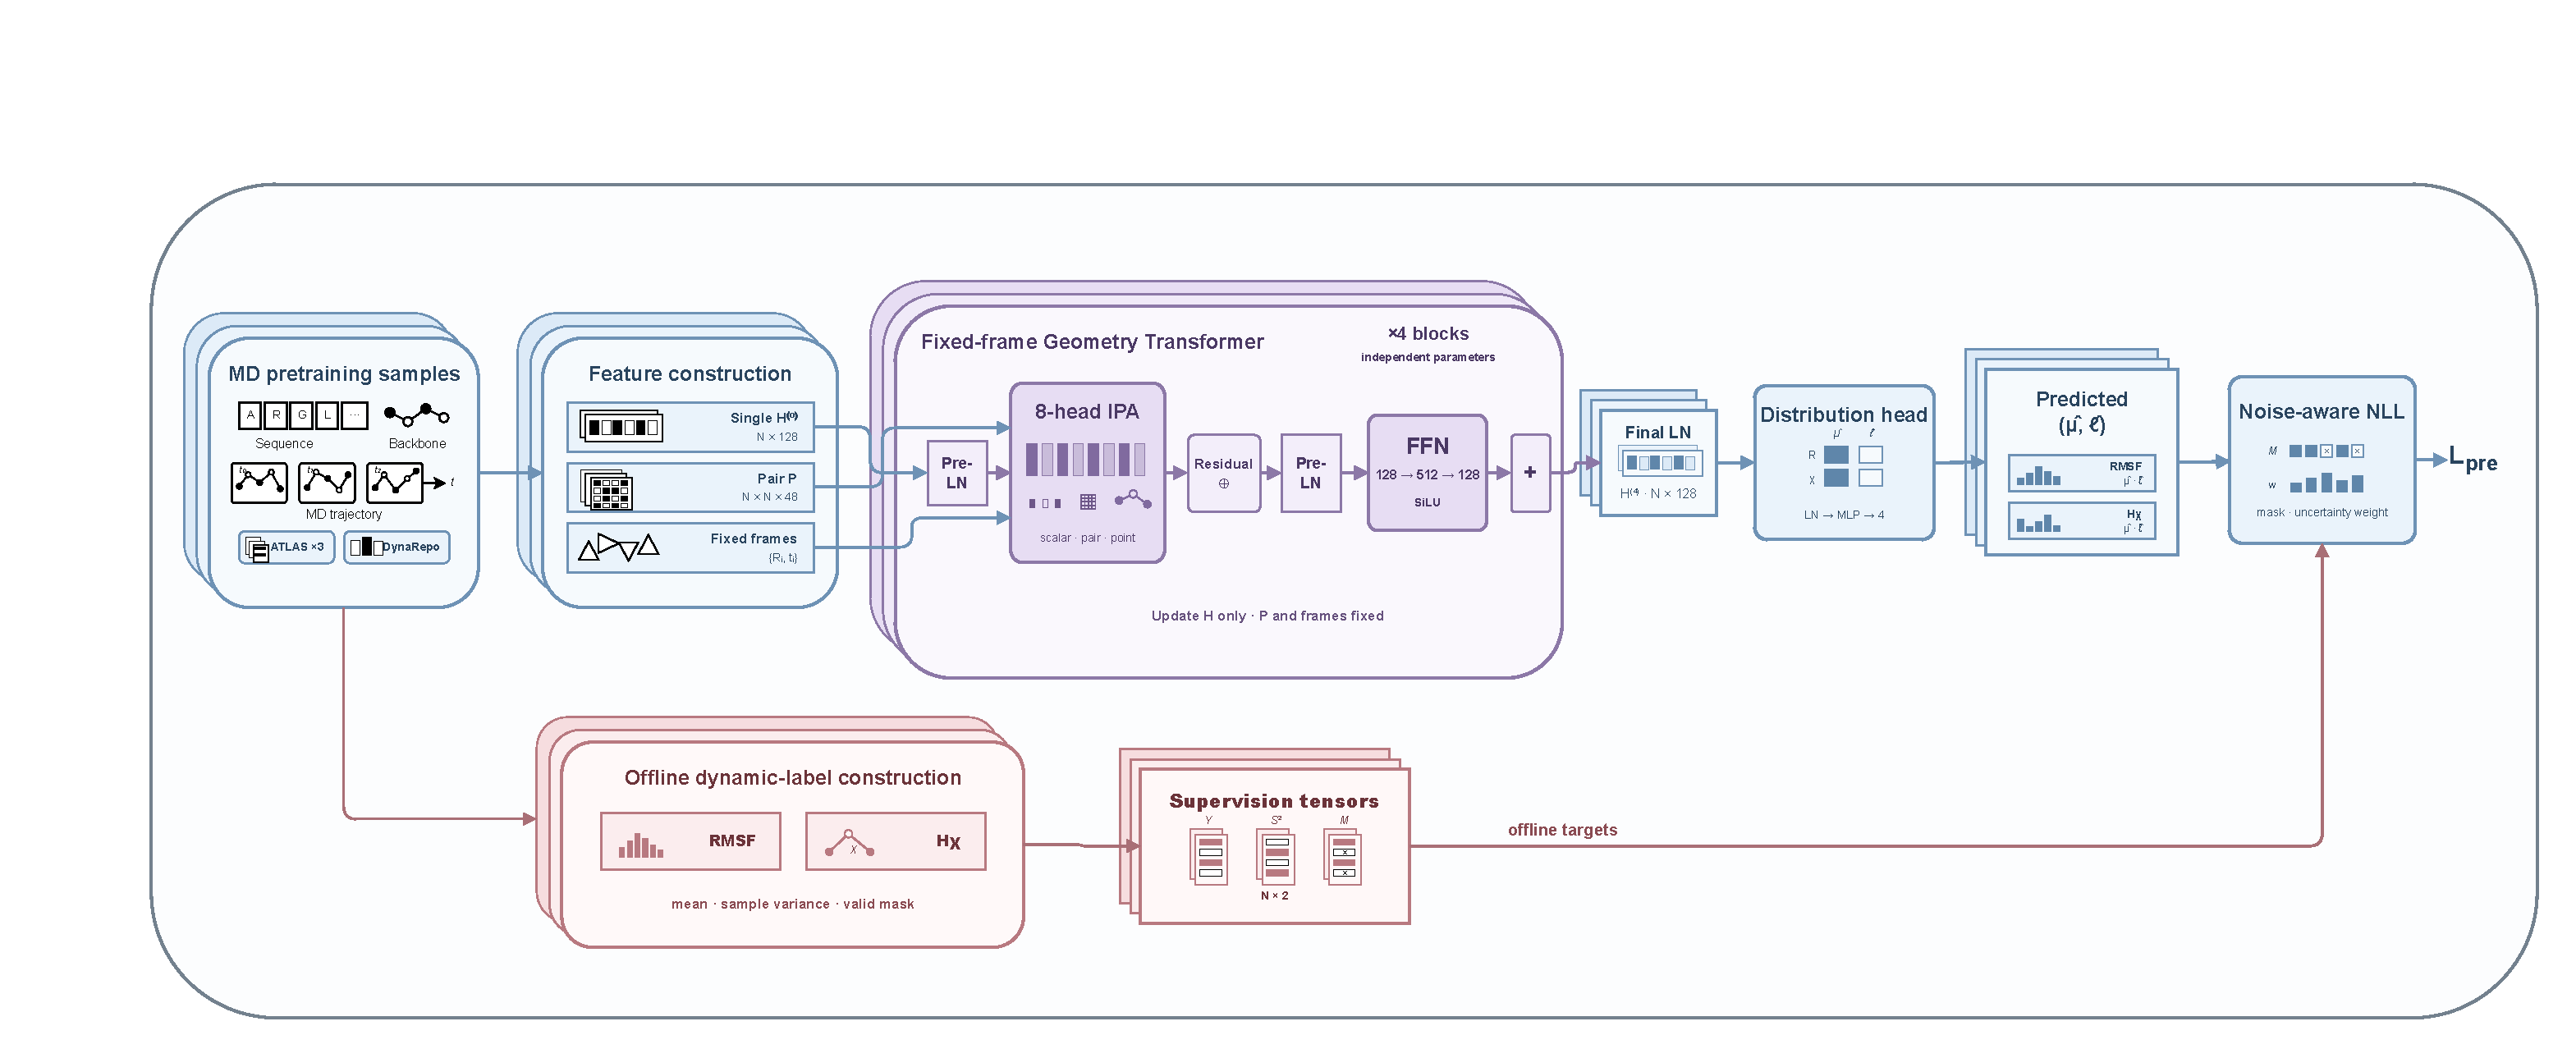
\includegraphics[width=\textwidth]{figures/f1_pipeline.pdf}
    \caption{\textbf{FlexPPI 绝对状态预训练流程。} 轨迹首先转换为逐残基 RMSF、
    侧链构象熵和 SASA 的标签均值、重复/窗口方差及有效掩码。静态结构分支构造
    氨基酸与条件表示、固定局部框架和残基对几何；四个具有独立参数的 IPA 模块在
    完整多链结构内传播标量、残基对和三维点信息。概率状态头输出三类动态量的均值
    与对数方差，并通过噪声感知负对数似然训练。}
    \label{fig:flexppi-pretraining}
\end{figure*}

当前模型使用两个独立的可学习氨基酸嵌入：主要序列嵌入
$\mathbf s_i\in\mathbb R^{128}$ 和辅助类型嵌入
$\mathbf a_i\in\mathbb R^{32}$。二者拼接并投影到 128 维。温度、轨迹时长和
数据来源组成条件向量
\begin{equation}
    \mathbf c=
    \left[\frac{T-300}{20},
    \frac{\log(1+t_{\mathrm{ns}})}{\log(501)},
    d_{\mathrm{set}}\right],
    \label{eq:condition-vector}
\end{equation}
其中 $d_{\mathrm{set}}=0$ 表示 ATLAS，$d_{\mathrm{set}}=1$ 表示 DynaRepo。
两层多层感知机将 $\mathbf c$ 映射为 128 维条件嵌入，初始残基表示为
\begin{equation}
    \mathbf h_i^{(0)}=
    \mathbf W_{\mathrm{in}}[\mathbf s_i\Vert\mathbf a_i]
    +\mathbf b_{\mathrm{in}}+\mathbf e^{\mathrm{cond}}.
    \label{eq:single-input}
\end{equation}
未知氨基酸保留为有效输入；批内填充位置和缺少有效主链框架的残基由掩码排除。

\subsubsection{固定局部框架与残基对几何}

对残基 $i$，以 C$\alpha$ 坐标为原点 $\mathbf t_i$，以 C$\alpha\rightarrow$C
方向为第一轴，将 C$\alpha\rightarrow$N 方向正交化为第二轴，并以叉乘得到第三轴，
构成旋转矩阵 $\mathbf R_i\in\mathbb R^{3\times3}$。缺少 N、C$\alpha$ 或 C 的
残基不参与几何注意力。对每个有序残基对 $(i,j)$，模型计算 C$\alpha$ 距离
$d_{ij}$、同链指示量、截断到 32 的残基编号间隔，以及在 $i$ 的局部框架中观察
$j$ 的单位方向
\begin{equation}
    \mathbf u_{ij}=
    \frac{\mathbf R_i^{\mathsf T}(\mathbf t_j-\mathbf t_i)}
    {\|\mathbf t_j-\mathbf t_i\|_2+\varepsilon}.
    \label{eq:local-direction}
\end{equation}
距离经 24 个中心均匀分布于 $0$--$24$~\AA{} 的径向基函数展开。原始几何特征
\begin{equation}
    \mathbf g_{ij}=
    \left[\boldsymbol\phi(d_{ij})\Vert
    \delta_{ij}^{\mathrm{chain}}\Vert
    \frac{\min(|r_i-r_j|,32)}{32}\Vert
    \mathbf u_{ij}\right]\in\mathbb R^{29}
    \label{eq:raw-pair-feature}
\end{equation}
由两层多层感知机投影为 $\mathbf p_{ij}\in\mathbb R^{48}$。距离和局部方向在
整体刚体变换下保持不变，因此残基对编码不依赖结构文件的全局坐标系。

\subsubsection{固定框架 IPA 与状态头}

四个 IPA 模块接收逐残基表示、残基对表示和固定框架。IPA 沿用
AlphaFold2\cite{jumper2021alphafold} 的基本构造：每个注意力头同时使用标量
查询--键相似度、残基对偏置和三维查询点--键点距离。对头 $h$，未归一化注意力
分数写为
\begin{equation}
    e_{ij}^{(h)}=
    \sqrt{\frac{1}{3d_h}}
    \langle\mathbf q_i^{(h)},\mathbf k_j^{(h)}\rangle
    +\sqrt{\frac{1}{3}}b^{(h)}(\mathbf p_{ij})
    -\frac{\gamma_h}{2}\sum_{r=1}^{P}
    \left\|
    \mathbf R_i\mathbf q_{ir}^{(h),\mathrm{pt}}+\mathbf t_i-
    \mathbf R_j\mathbf k_{jr}^{(h),\mathrm{pt}}-\mathbf t_j
    \right\|_2^2,
    \label{eq:ipa-logit}
\end{equation}
其中 $d_h=16$、$P=4$，$\gamma_h$ 为可学习的非负点距离权重。对有效残基 $j$
执行 softmax 后，注意力权重同时聚合 16 维标量值、48 维残基对值和 8 个三维
值点；三维聚合结果转换回查询残基的局部框架。每个模块包含 8 个头，并采用标准
Transformer\cite{vaswani2017attention} 的预归一化、残差连接和逐位置前馈网络。
局部框架和坐标在四层编码过程中固定，网络只更新逐残基隐藏表示。

最终状态头对 128 维残基表示执行 LayerNorm、线性变换和 SiLU 激活，输出三组
均值与对数方差。均值经 softplus 约束为非负；对数方差截断至 $[-8,6]$。因此
两个输出张量的形状均为 $N\times3$。

\subsection{噪声感知目标与训练设置}

对残基 $i$ 和指标 $k$，模型方差为 $\exp(\hat\ell_{ik})$，标签重复方差为
$s_{ik}^{2}$。二者相加后使用异方差高斯负对数似然：
\begin{equation}
    \ell_{ik}=\frac{1}{2}\left[
    \frac{(\hat\mu_{ik}-y_{ik})^2}
    {\exp(\hat\ell_{ik})+s_{ik}^{2}}
    +\log\left(\exp(\hat\ell_{ik})+s_{ik}^{2}\right)
    \right].
    \label{eq:pretraining-nll}
\end{equation}
第一项降低高噪声标签对均值误差的权重，第二项防止模型仅通过增大预测方差降低
损失。总方差截断到 $[10^{-6},10^6]$。令 $m_{ik}$ 同时表示目标残基、标签存在、
非填充和局部框架有效，则
\begin{equation}
    \mathcal L_{\mathrm{pre}}=
    \frac{\sum_{i,k}m_{ik}w_k\ell_{ik}}
    {\max(\sum_{i,k}m_{ik}w_k,1)},
    \qquad
    (w_{\mathrm{RMSF}},w_\chi,w_{\mathrm{SASA}})=(1,0.5,0.25).
    \label{eq:pretraining-loss}
\end{equation}

ATLAS 与 DynaRepo 清单合并后，划分程序依次尝试按同源簇、PDB 和样本标识分组；
当前清单缺少前两类字段，因此实际按样本标识、固定随机种子 7 划分 10\% 验证集。
该划分不是同源隔离测试，故内部结果仅作模型选择和能力诊断。预训练使用 4 层、
8 头 IPA，残基表示维度 128、残基对维度 48、dropout 0.1、批大小 1 和最大长度
768；模型训练 20 个 epoch，采用 AdamW，学习率 $3\times10^{-4}$、权重衰减
$10^{-4}$，梯度范数截断为 1.0，并保存验证损失最低的检查点。

% !TeX root = ../paper.tex

\section{实验}

\subsection{实验状态与证据等级}

本文使用 ``已完成''、``进行中'' 和 ``计划'' 三种状态。已完成结果均来自
仓库中可重建的 JSON/CSV 产物；但当前训练器没有完全未接触的测试划分，内部
验证集参与了最优 checkpoint 选择，因此这些结果只用于能力诊断，不能写成
独立测试或 state-of-the-art。表 \ref{tab:experiment-status} 汇总了当前状态。

% !TeX root = ../paper.tex

\begin{table}[!ht]
  \centering
  \caption{实验完成状态与可作出的结论。}
  \label{tab:experiment-status}
  \small
  \begin{tabularx}{\textwidth}{
    >{\raggedright\arraybackslash}p{3.2cm}
    >{\raggedright\arraybackslash}p{1.5cm}
    X}
    \toprule
    实验 & 状态 & 当前证据或完成条件 \\
    \midrule
    ATLAS/\allowbreak DynaRepo 动态标签流水线 & 已完成 &
      RMSF、侧链构象熵、SASA、标签方差与残基映射均已有可重建产物。\\
    绝对状态内部验证 & 已完成 &
      276 个系统；验证集参与 checkpoint 选择，只能作内部诊断。\\
    FastProtFlex 共同任务 & 已完成 &
      ATLAS 191 个蛋白、DynaRepo 31 个单链和 54 个复合体；比较相对排序。\\
    apo/holo 配对响应 & 已完成 &
      7 个模型选择验证体系；$\Delta$RMSF 仅有弱增益，尚无独立测试。\\
    ITrace 外部 MD 测评 & 已完成 &
      245 个 TCR--pMHC、735 条轨迹；排除 3KXF 后主队列为 244 个复合体；
      已直接检验完整体模型能否预测 MD 的肽内残基排序、九肽位置模式和接触
      差异，并另行完成 pMHC、TCR 二聚体和五条孤立链的
      RMSF/$H_\chi$/SASA 上下文消融。\\
    序列/结构近同源审计 & 计划 &
      需要对 ITrace 与全部训练链执行 MMseqs2、Foldseek 及折叠层级隔离。\\
    独立 apo/holo 响应测试 & 计划 &
      需要从训练和选轮次中隔离，并补齐成对 $\Delta$SASA。\\
    复合物 $\Delta G_{\mathrm{bind}}$ 微调 & 计划 &
      需要真实亲和力标签、A/B 对称亲和力头和静态/动态消融。\\
    突变 $\Delta\Delta G$ 微调 & 计划 &
      需要 WT/突变配对标签、正反反对称约束和家族/界面隔离测试。\\
    \bottomrule
  \end{tabularx}
\end{table}


\subsection{评价协议}

绝对状态任务先在每个蛋白内计算 Pearson、Spearman、MAE、RMSE 和一致性相关
系数，再让每个蛋白等权平均；所有残基混合计算的 pooled 指标只作补充，避免
长蛋白支配结果。将每个蛋白真实 RMSF 最高的 20\% 残基定义为高柔性集合，
报告 AUROC、average precision（AP）和 Precision@K。配对响应除回归指标外，
在 RMSF 和侧链熵上使用 0.1 的 dead zone，把残基分成刚化、中性和增柔三类，
报告 macro-F1、真实活跃残基的符号准确率以及绝对变化最大 20\% 残基的检出。
所有置信区间均以蛋白或复合体为重采样单位进行配对 bootstrap。

\subsection{已经完成：标签流水线与绝对状态诊断}

ATLAS 的 1,938 个体系已经全部完成索引，包含 444,240 个具有三重复 RMSF 的
残基；DynaRepo 的 922 个体系包含 366,777 个 RMSF、294,358 个侧链构象熵和
51,459 个 SASA 标签。当前绝对状态验证包含 276 个系统。表
\ref{tab:state-head-results} 表明预训练模型已经学习到稳定的蛋白内柔性排序，
其中侧链构象熵最强；但是配对响应微调使 RMSF 和侧链熵下降，并使稀疏的 SASA
任务发生灾难性遗忘。这一结果支持在后续亲和力训练中冻结底层表示、回放旧任务
并采用多目标 checkpoint 选择。

% !TeX root = ../paper.tex

\begin{table}[htbp]
  \centering
  \caption{绝对状态头在模型选择验证集上的结果。``系统/残基''为相应标签的
  有效数量；这些结果不是未接触测试。}
  \label{tab:state-head-results}
  \small
  \resizebox{\textwidth}{!}{%
  \begin{tabular}{llrrrrr}
    \toprule
    标签 & 检查点 & 系统/残基 & MAE &
    pooled Pearson & 蛋白等权 Spearman & top-20\% AP \\
    \midrule
    RMSF & 预训练 & 276 / 66,464 & $0.535\,\text{\AA}$ & 0.701 & 0.811 & 0.786 \\
    RMSF & 响应微调 & 276 / 66,464 & $0.592\,\text{\AA}$ & 0.679 & 0.750 & 0.743 \\
    $H_\chi$ & 预训练 & 85 / 21,870 & 0.201 & 0.958 & 0.928 & 0.939 \\
    $H_\chi$ & 响应微调 & 85 / 21,870 & 0.212 & 0.951 & 0.919 & 0.933 \\
    SASA & 预训练 & 11 / 4,028 & $16.80\,\text{\AA}^2$ & 0.871 & 0.871 & 0.801 \\
    SASA & 响应微调 & 11 / 4,028 & $76.88\,\text{\AA}^2$ & $-0.168$ & $-0.096$ & 0.234 \\
    \bottomrule
  \end{tabular}%
  }
\end{table}


\subsection{已经完成：与 FastProtFlex 的共同静态任务}

FastProtFlex 输出每条蛋白内部标准化的相对柔性，不能参加以
$\text{\AA}$ 为单位的绝对 MAE 比较。表 \ref{tab:rmsf-results} 因而只报告两种
方法都能回答的排序、标准化误差和高柔性检出。ATLAS 的 191 个共同蛋白上，
FlexPPI 的蛋白等权 Spearman 为 0.8205，FastProtFlex 为 0.7984；DynaRepo
单链和复合体也得到同方向差异。复合体分层进一步显示，FlexPPI 的总体优势主要
来自非界面区域，界面 Spearman 尚未超过 FastProtFlex，因此不能宣称已经解决
界面柔性预测。ATLAS 参与了两种模型的开发，DynaRepo 又存在训练域不对称，
这些比较仍属于同域诊断。

% !TeX root = ../paper.tex
% 所有方法均在冻结的共同残基集合上计算；加粗为每个数据集的最优值。
% FlexPPI 行以浅灰底色突出；面板按 DynaRepo 复合体、DynaRepo 单链、
% ATLAS 单链排列，ATLAS 为开发域参考。
\begin{table}[htbp]
  \centering
  \caption{七种方法在共同静态 RMSF 任务上的体系等权结果。浅灰行为本文方法
  FlexPPI；BackFlip 与 FastProtFlex 对复合体逐链独立预测，ProDy、RMSF-net-PDB
  与 FlexPPI 读取完整复合体。ProDy、RMSF-net-PDB 和 FastProtFlex 仅给出相对
  涨落，故主表统一比较排序、链内标准化误差与高柔性残基检出；ATLAS 属于多个
  学习模型的开发域，不作为外部测试。}
  \label{tab:rmsf-results}
  \scriptsize
  \resizebox{\textwidth}{!}{%
  \begin{tabular}{llrrrrrr}
    \toprule
    数据集 & 方法 &
    Spearman $\uparrow$ & Pearson $\uparrow$ &
    z-MAE $\downarrow$ & AUROC $\uparrow$ &
    AP $\uparrow$ & P@K $\uparrow$ \\
    \midrule
    \rowcolor{gray!12} \cellcolor{white}\multirow{7}{*}{DynaRepo 复合体} & FlexPPI
      & \textbf{0.7902} & \textbf{0.7506} & \textbf{0.4490}
      & \textbf{0.9042} & \textbf{0.7620} & \textbf{0.6730} \\
    & FastProtFlex
      & 0.7599 & 0.6930 & 0.5549 & 0.8926 & 0.7374 & 0.6509 \\
    & BackFlip-seq
      & 0.7460 & 0.7366 & 0.4563 & 0.8934 & 0.7470 & 0.6536 \\
    & BackFlip-structure
      & 0.7336 & 0.7143 & 0.4773 & 0.8829 & 0.7190 & 0.6259 \\
    & ProDy-ANM
      & 0.6112 & 0.5315 & 0.5716 & 0.8032 & 0.6443 & 0.5509 \\
    & ProDy-GNM
      & 0.5440 & 0.5194 & 0.5760 & 0.7941 & 0.6485 & 0.5740 \\
    & RMSF-net-PDB
      & 0.5494 & 0.5428 & 0.6587 & 0.7943 & 0.6054 & 0.5387 \\
    \midrule
    \rowcolor{gray!12} \cellcolor{white}\multirow{7}{*}{DynaRepo 单链} & FlexPPI
      & \textbf{0.8517} & 0.7854 & 0.4088
      & \textbf{0.9212} & \textbf{0.7835} & \textbf{0.7040} \\
    & BackFlip-seq
      & 0.8345 & \textbf{0.7872} & \textbf{0.3988}
      & 0.9198 & 0.7776 & 0.6967 \\
    & FastProtFlex
      & 0.8298 & 0.7476 & 0.5032 & 0.9134 & 0.7678 & 0.6903 \\
    & BackFlip-structure
      & 0.8253 & 0.7618 & 0.4241 & 0.9106 & 0.7646 & 0.6757 \\
    & ProDy-ANM
      & 0.8080 & 0.6046 & 0.5102 & 0.9006 & 0.7519 & 0.6670 \\
    & ProDy-GNM
      & 0.7642 & 0.6214 & 0.5270 & 0.8920 & 0.7434 & 0.6635 \\
    & RMSF-net-PDB
      & 0.6735 & 0.6554 & 0.5682 & 0.8541 & 0.6733 & 0.6137 \\
    \midrule
    \rowcolor{gray!12} \cellcolor{white}\multirow{7}{*}{ATLAS 单链} & FlexPPI
      & 0.8205 & 0.8509 & 0.3393 & 0.9230 & 0.8024 & 0.7069 \\
    & BackFlip-seq
      & \textbf{0.8362} & \textbf{0.8830} & \textbf{0.3023}
      & \textbf{0.9362} & \textbf{0.8309} & \textbf{0.7363} \\
    & BackFlip-structure
      & 0.8083 & 0.8575 & 0.3317 & 0.9162 & 0.7953 & 0.7050 \\
    & FastProtFlex
      & 0.7984 & 0.7717 & 0.4870 & 0.9125 & 0.7821 & 0.6898 \\
    & ProDy-ANM
      & 0.7897 & 0.6882 & 0.4446 & 0.8948 & 0.7648 & 0.6736 \\
    & ProDy-GNM
      & 0.7415 & 0.7268 & 0.4402 & 0.8891 & 0.7526 & 0.6660 \\
    & RMSF-net-PDB
      & 0.6682 & 0.7012 & 0.5341 & 0.8591 & 0.6890 & 0.6106 \\
    \bottomrule
  \end{tabular}%
  }
\end{table}


\subsection{已经完成：配对响应诊断}

当前 test53 配对清单中 37 对全部参与微调流程，模型选择验证只含 7 个体系、
2,124 个有效 $\Delta$RMSF 残基和 1,691 个有效
$\Delta H_\chi$ 残基。表 \ref{tab:response-results} 显示，直接响应头把
$\Delta$RMSF MAE 从零变化的 $0.221\,\text{\AA}$ 降到
$0.209\,\text{\AA}$，改善 5.2\%，且比两个状态直接相减的
$0.275\,\text{\AA}$ 更低；然而逐蛋白 Spearman 只有 0.160，活跃残基符号
准确率为 34.3\%，增柔类别 F1 只有 0.063。$\Delta H_\chi$ 响应头的 MAE
还差于零变化基线，当前也没有配对 $\Delta$SASA 标签。因此，模型目前只对
$\Delta$RMSF 提供弱的平均误差增益，尚未可靠学会变化方向或强变化尾部。

% !TeX root = ../paper.tex

\begin{table}[htbp]
  \centering
  \caption{配对响应在 7 个模型选择验证体系上的内部诊断。相对零变化改善为
  正值时表示 MAE 降低。}
  \label{tab:response-results}
  \small
  \resizebox{\textwidth}{!}{%
  \begin{tabular}{llrrrrr}
    \toprule
    标签 & 方法 & MAE & Pearson & Spearman &
    相对零变化 MAE 改善 & 活跃残基符号准确率 \\
    \midrule
    $\Delta$RMSF & 响应头 & $0.209\,\text{\AA}$ & 0.236 & 0.197 & $+5.2\%$ & 34.3\% \\
    $\Delta$RMSF & 状态相减 & $0.275\,\text{\AA}$ & 0.293 & 0.171 & $-24.7\%$ & 37.5\% \\
    $\Delta$RMSF & 零变化 & $0.221\,\text{\AA}$ & -- & -- & 0 & 0\% \\
    $\Delta H_\chi$ & 响应头 & 0.139 & 0.176 & 0.046 & $-3.9\%$ & 2.7\% \\
    $\Delta H_\chi$ & 状态相减 & 0.145 & 0.234 & 0.082 & $-8.8\%$ & 15.2\% \\
    $\Delta H_\chi$ & 零变化 & 0.133 & -- & -- & 0 & 0\% \\
    \bottomrule
  \end{tabular}%
  }
\end{table}


\subsection{已经完成：TCR3D 外部代理}

在排除精确训练 PDB 重叠后，TCR3D 共成功评测 1,189 条 TCR $\alpha/\beta$
链和 129,268 个残基。预测 RMSF 与晶体 B-factor 换算代理的每链等权
Spearman 为 0.389，95\% bootstrap 区间为 $[0.378,0.397]$；识别 CDR3
相对框架区的 pooled AUROC 为 0.612、AP 为 0.332，而随机 AP 为 0.144。
该结果说明模型保留了中等程度的跨域局部排序信号，但 B-factor 同时受到晶格、
分辨率和精修影响，TCR3D 也没有配对 MD，故本实验不能作为 MD-RMSF 或结合
响应真值。将数据域编码从 ATLAS 改为 DynaRepo 时，RMSF 平均绝对漂移达到
$0.278\,\text{\AA}$，说明后续应删除数据集身份这一非物理条件，改用温度、
离子强度、力场和时间窗等可测变量。

\begin{figure}[!htbp]
  \centering
  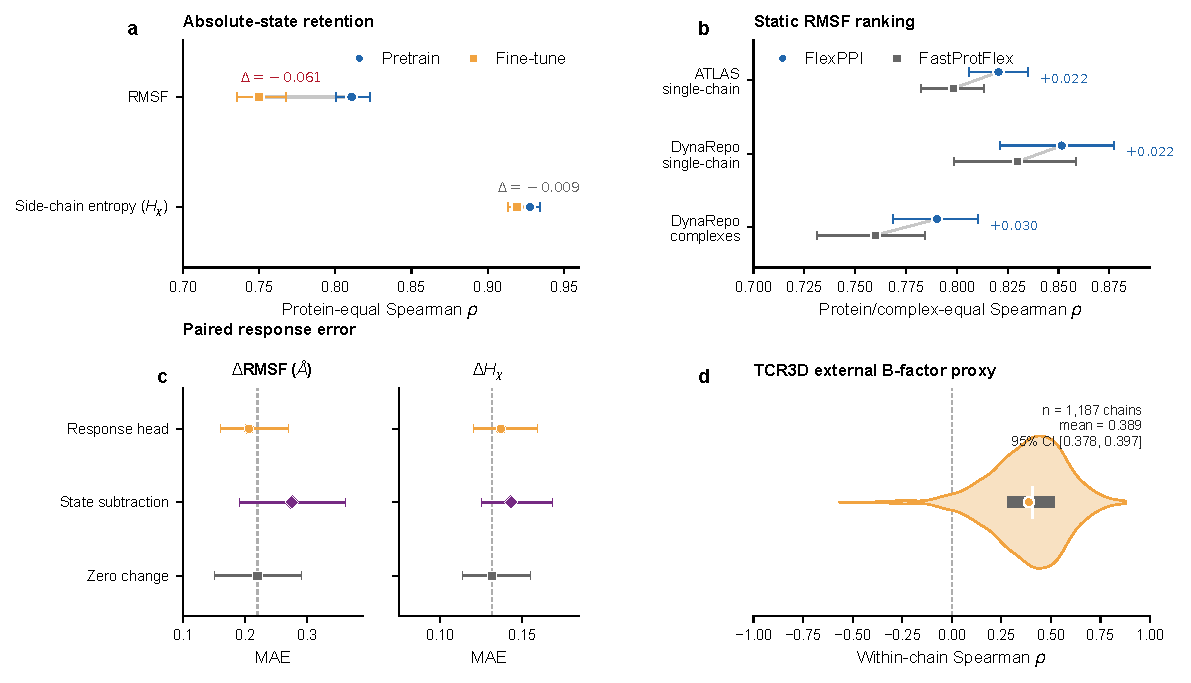
\includegraphics[width=\textwidth]{fig_completed_experiments.pdf}
  \caption{已完成柔性实验的统一可视化。所有点估计均先在单个蛋白、复合物或体系
  内计算，再对体系等权平均；误差线为归档结果中的非参数 bootstrap 95\% 置信
  区间。（a）预训练与配对响应微调后的绝对状态预测能力，仅展示 RMSF 与侧链
  构象熵 $H_\chi$，差值定义为微调减预训练。（b）FlexPPI 与 FastProtFlex
  在共同可回答的静态 RMSF 排序任务上的比较，右侧数字为
  $\rho_{\mathrm{FlexPPI}}-\rho_{\mathrm{FastProtFlex}}$。（c）7 个配对体系上
  响应头、状态相减和零变化基线的体系等权 MAE；竖虚线对应零变化基线，误差线
  反映当前小样本下的不确定性。（d）TCR3D 中 1,187 条可计算相关性的链的
  B-factor 代理 Spearman 分布；橙色点为链等权均值，灰色线为其 95\% 置信
  区间。TCR3D 共评测 1,189 条链，其中 2 条因代理值或预测值为常数而不能计算
  Spearman。面板（a）--（c）属于内部验证或模型选择诊断，面板（d）使用晶体
  B-factor 代理而非 MD 真值，因而均不作为独立测试集上的最终性能声明。}
  \label{fig:completed-experiments}
\end{figure}
\clearpage

\subsection{必须补做：冻结的外部柔性测试}

正式柔性结论需要建立完全未参与训练、调参和 checkpoint 选择的外部 MD 测试集。
候选体系在进入测试前必须同时与全部训练链进行 MMseqs2 序列搜索以及
Foldseek/CATH/ECOD 结构拓扑搜索，至少剔除高于 30\% 序列一致性的近同源，
并分别报告 ``新序列但旧折叠'' 和 ``新折叠''。每个体系应包含不少于三条独立
初速度的重复轨迹，在统一温度、力场、水模型、离子条件、平衡流程和生产时长下
生成标签；重复 A 对重复 B 的性能作为经验噪声上限。所有方法统一使用
$C_\alpha$、链级 Kabsch 对齐、共同残基掩码和缺失残基规则。

第一轮必须运行常数、氨基酸类型、二级结构、SASA、反向 pLDDT、GNM、ANM、
CABS-flex、FastProtFlex、FlexPred-SVR、PEGASUS、Flexpert-Seq 和
Flexpert-3D。第二轮加入 BackFlip、RocketSHP 和 RMSF-net 的 PDB-only 分支。
绝对输出模型参加 MAE/RMSE/CCC；相对输出模型只参加每蛋白相关、排序和
top-$k$ 检出。BackFlip 的局部对齐标签与 FlexPPI 的链级对齐标签分开报告，
RMSF-net 完整 cryo-EM 模型进入额外实验信息轨道。

\subsection{必须补做：独立 apo/holo 响应测试}

需要重新冻结一套从未进入响应微调和轮次选择的 apo/holo 测试集，并补齐两态
RMSF、侧链熵和 SASA 标签。界面定义从当前的跨链
$C_\alpha\leq8\,\text{\AA}$ 升级为任意重原子
$\leq5\,\text{\AA}$，另设 $5$--$12\,\text{\AA}$ 近界面和远端变构区域。
响应头、状态相减和零变化三种方法并列；每种训练至少使用五个随机种子，报告
蛋白级 bootstrap 区间、配对显著性检验、方向 macro-F1、强变化 AP、推理时间
和失败样本。还需比较冻结编码器、顶部小学习率解冻、旧任务 replay 和多任务
checkpoint 选择，以确定哪种方案能在学习响应时保留绝对状态能力。

\subsection{计划实验：由柔性响应预测结合亲和力}

亲和力实验分成两个任务。任务一预测复合物的
$\Delta G_{\mathrm{bind}}^{\circ}$；任务二预测突变或条件变化造成的
$\Delta\Delta G$。所有 $K_d/K_i$ 标签转换为统一的
$\mathrm{kcal\,mol^{-1}}$，保存温度、pH、离子强度、测量方法和不等式标签；
无法确定温度的样本单列或使用带缺失条件的模型，不能静默假设所有实验等价。
数据划分以复合物家族和界面相似性为单位，任何相同或近同源链、相同界面模板
及同一突变的正反记录不得跨越训练、验证和测试。

对每个样本按式 \eqref{eq:two-sided-response} 生成 A、B 双侧特征。主模型使用
式 \eqref{eq:symmetric-pooling} 的 A/B 对称表示；第一阶段冻结 FlexPPI，
只训练亲和力头，第二阶段小学习率解冻顶部表示块并保留
$\mathcal L_{\mathrm{pair}}$。主指标为复合物等权 MAE、RMSE、Pearson、
Spearman、$R^2$、CCC 和预测区间覆盖率；$\Delta\Delta G$ 另外报告稳定化/
去稳定化方向准确率、macro-F1 和反向反对称误差。

亲和力消融至少包含：（1）仅静态界面几何与理化特征；（2）仅绝对 RMSF、
侧链熵和 SASA；（3）仅直接柔性响应；（4）仅状态相减；（5）仅残基隐藏表示；
（6）静态与动态全部特征；（7）逐一移除 RMSF、侧链熵或 SASA；（8）真实
apo/holo 与从复合体删除伙伴的伪 apo 对照；（9）预训练状态 checkpoint、
响应微调 checkpoint 和带 replay 的联合 checkpoint。只有当 ``静态+动态''
在冻结同源/界面测试集上稳定超过 ``仅静态''，且多个随机种子的改进置信区间
不跨零，才能声称柔性响应为亲和力预测提供了增量价值。

% !TeX root = ../paper.tex

\section{讨论}

\subsection{伙伴上下文提供了信息，但其作用不是局部一致改进}

FlexPPI 在 ITrace 全结构上的平均排序优于逐链 FastProtFlex，也优于同一检查点的
孤立链输入。这一结果说明，多链结构中确实存在单链模型无法利用的信息。分层分析
同时表明，该信息主要改善非界面和整体结构范围的排序，而不是直接提高接触残基的
预测准确性。完整输入在非界面的 Spearman 增益为正，在界面则为负；绝对 MAE 也
随伙伴加入略有上升。因此，“模型利用了复合物上下文”和“模型正确学习了界面
动力学”是两个不同命题，整体相关系数只能支持前者。

固定坐标消融解释了这种分离。加入伙伴后，模型对几乎所有非肽界面残基都施加负向
RMSF 修正，并在肽中央 P4--P8 同步降低 RMSF、$H_\chi$ 和 SASA。该响应与重原子
接触距离高度相关，说明局部几何已进入表示；但模型将“接触导致受限”近似为单向
规则，没有充分表示界面两侧的链别差异。对 MHC 接触面，这一规则与 MD 中的相对
刚性一致；对 TCR$\beta$ 接触面及 CDR1/2$\beta$，相同规则却抹除了真实的相对
柔性。该结果提示，下一代模型不应只加强跨链注意力，还需要能够在相同接触几何下
区分伙伴角色、残基化学环境和潜在增柔机制。

\subsection{残基级外部评估比群体平均模式更严格}

九肽群体均值的 Pearson 达到 0.684，容易形成模型已恢复肽动力学图景的印象；然而，
逐复合体平均 Spearman 仅为 0.302，最活跃残基命中率为 34.0\%。二者的差异来自
评价粒度：群体均值主要检验模型是否学到肽位置的平均先验，逐复合体指标则要求模型
识别同一位置在不同 TCR--pMHC 环境中的变化。类似地，模型预测的接触残基在队列
平均上更刚，但这一方向在单个复合体中只略高于随机比例。对需要选择突变位点或实验
测量位点的应用，逐体系残基定位比群体均值更接近实际决策目标，应被视为主要证据。

7L1D/7RRG 个案和氨基酸类型残差可用于生成后续假设，但不能提高外部准确性的证据
等级。前者证明同一肽中央段响应可在两个结构背景中内部复现，后者显示侧链构象熵
比主链 RMSF 更依赖残基类型；两项分析均缺少配对 $H_\chi$/SASA 真值。本文因而
将它们保留为模型可解释性结果，而不表述为已经验证的 TCR 识别机制。

\subsection{上下文响应、结合响应与结合自由能的边界}

从完整复合物中删除伙伴会同时改变跨链边、输入长度和全局注意力的归一化集合；保留
结构仍处于结合态构象。由此得到的差值反映模型对输入上下文的敏感性，而不是蛋白质
从游离态到结合态的物理路径。抗体 CDR 的结构分析已表明，局部环构象改变、环相对
框架移动和构象选择需要分别定义\cite{liu2024cdr}；同理，真实动态响应需要两态
独立结构及轨迹，不能由删链操作替代。

逐残基柔性变化也不能直接换算为结合亲和力。标准结合自由能取决于结合态与游离态
自由能之差，并共同包含相互作用焓、溶剂重排、构象集合、平移和转动熵等贡献。
RMSF 不包含残基间运动协方差，$H_\chi$ 只覆盖离散化的侧链扭转角，SASA 也不区分
被埋藏表面的化学组成。现有热力学约束模型必须显式比较结合/游离状态或完整热力学
循环\cite{jiao2024boltzmann}。因此，FlexPPI 的三类输出可以作为亲和力模型的候选
特征，但不能通过“刚化越强、亲和力越高”的固定规则得到 $\Delta G$。

\subsection{局限性}

本研究存在五项主要限制。第一，ITrace 主队列排除了精确 PDB 重叠，但尚未对全部
训练链完成 MMseqs2 序列近同源和 Foldseek/CATH/ECOD 结构近同源审计；当前证据
不能上升为新折叠泛化。第二，235/245 个 ITrace 复合体超过预训练长度上限 768，
完整输入和孤立输入又处于不同长度范围，因而上下文差值可能包含长度外推效应。
第三，ITrace 仅为 RMSF 提供外部真值，模型的 $H_\chi$ 与 SASA 响应尚未得到同一
体系的 MD 验证。第四，配对响应数据仅有 37 对，全部进入微调，7 个验证体系还用于
检查点选择；该实验没有独立测试集，也未覆盖多个随机种子。第五，当前比较集中于
FastProtFlex，尚缺少 GNM、ANM、CABS-flex、Flexpert-Seq/Flexpert-3D 等不同原理
方法在完全一致输入和残基集合上的系统基准。

\subsection{后续工作}

后续验证应优先解决证据独立性，而非继续增加模型复杂度。第一步是在全部训练数据与
ITrace 之间完成序列和结构去同源，并分别报告“新序列但旧折叠”与“新折叠”结果；
同时进行长度分层并补充物理和学习型基线。第二步是建立从未参与训练或轮次选择的
apo/holo 多重复轨迹测试集，同时计算 $\Delta$RMSF、$\Delta H_\chi$ 和
$\Delta$SASA；响应头、状态相减和零变化基线应在多随机种子下比较。第三步是在响应
微调中加入绝对状态 replay、多目标检查点选择和角色感知的跨链表示，以减少 SASA
遗忘和单向刚化偏置。

只有在上述状态与响应能力被独立验证后，才适合训练复合物级亲和力头。该阶段应以
真实 $K_d/K_i$ 转换的 $\Delta G_{\mathrm{bind}}^{\circ}$ 或成对
$\Delta\Delta G$ 为监督，按复合物家族和界面模板隔离数据，并直接比较“仅静态
界面特征”与“静态特征加 FlexPPI 动态表示”。只有后者在隔离测试集和多个随机种子
上稳定改进，才能将柔性表示解释为亲和力预测的增量信息。

% !TeX root = ../paper.tex

\section{结论}

本文提出 FlexPPI，以主链局部框架和不变点注意力构建对整体旋转和平移保持不变的
几何表示，并从静态多链结构预测逐残基 RMSF、侧链构象熵、SASA 及其不确定性；模型在训练完成后使用 ITrace TCR--pMHC 轨迹进行
外部评估。排除精确 PDB 重叠后，模型在 244 条抗原肽内的平均残基 Spearman 为
0.302，能够恢复部分九肽位置先验和队列平均接触信号，但最活跃残基命中率仅为
34.0\%。完整复合物在全部链上的平均 Spearman 为 0.740，高于逐链 BackFlip-seq
的 0.704、FastProtFlex 的 0.685 和 RMSF-net-PDB 的 0.526，也高于
ProDy-ANM/GNM；但 BackFlip-seq 在线性相关和标准化误差上更好，结构版 BackFlip
在 CDR3 内达到 0.920，超过 FlexPPI 的 0.812。分层结果表明，FlexPPI 的总体排序
优势主要来自非界面、TCR framework 和抗原肽，而不是所有界面区域。

固定坐标伙伴消融揭示了模型利用伙伴信息的方式：相对于只删除对侧伙伴且保留内部
组成的 pMHC/TCR 子复合物，完整输入将 RMSF Spearman 从 0.691 提高至 0.740，
绝对 MAE 从 $0.373\,\text{\AA}$ 降至 $0.346\,\text{\AA}$；全部保留原子的坐标
差为零。加入伙伴同时在接触区域产生强烈且可定位的负向修正，直接接触残基相对
非接触残基额外降低 $0.242\,\text{\AA}$ RMSF、0.225 的 $H_\chi$ 和
$22.87\,\text{\AA}^2$ SASA。该修正在 MHC 接触面方向正确，却错误压低了 TCR 接触面以及
CDR1/2$\beta$ 的柔性，并缩小了 CDR3$\alpha$ 与 CDR3$\beta$ 的链间差异。
因此，FlexPPI 已学到伙伴接触约束，但这一约束过度单向，尚不能稳定刻画界面两侧
及不同 TCR 链的动力学分工。

本文结果同时限定了模型输出的物理解释。共享结合态坐标的删链差值只能表示上下文
响应；缺少独立 apo/holo 轨迹时，不能称为结合诱导动态变化。RMSF、侧链构象熵和
SASA 也不能直接等同于结合自由能。FlexPPI 的当前价值在于以低成本提出残基级动态
假设并暴露静态几何模型的能力边界。完成去同源外部测试、独立配对轨迹验证和构象
采样型基线比较后，方可进一步判断这些动态表示能否为结合响应或亲和力预测提供
可靠增量。

% !TeX root = ../paper.tex

\appendix
\section{ITrace 补充分析}

\begin{figure}[H]
  \centering
  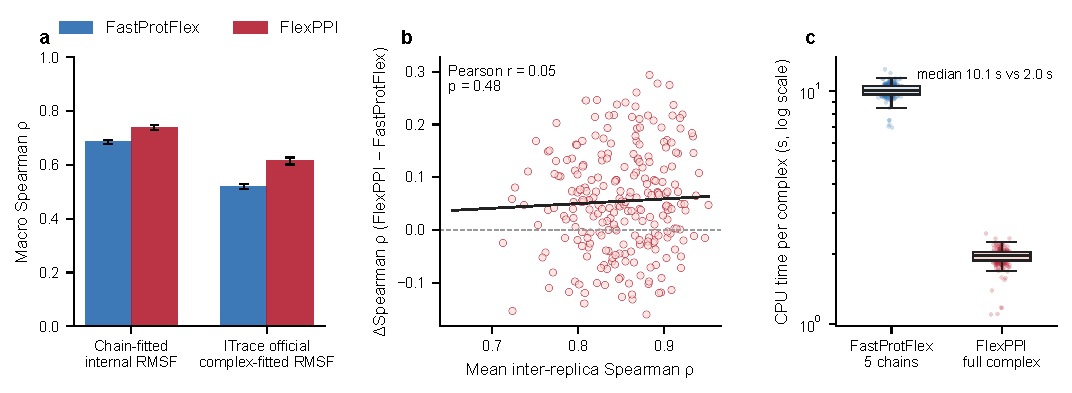
\includegraphics[width=\textwidth]{fig_itrace_sensitivity.pdf}
  \caption{ITrace 标签定义与样本纳入规则的敏感性分析。主分析使用逐链拟合的
  $C_\alpha$ RMSF，并排除唯一精确训练 PDB 重叠 3KXF；次分析改用 ITrace
  官方全复合体拟合标签，或把 3KXF 加回全部 245 个复合体。逐链拟合标签减少
  链间整体运动对链内柔性的污染；两种纳入规则下总体排序不变，而官方标签下
  FlexPPI 相对 FastProtFlex 的优势更大，说明主要结论并非由单一样本或单一
  对齐定义造成。误差线为 2,000 次复合体 bootstrap 95\% 置信区间。}
  \label{fig:itrace-sensitivity}
\end{figure}

\subsection{轨迹覆盖、预测成功率与标签质量控制}

本研究使用的 ITrace 数据快照包含 245 个复合体和 735 条轨迹，即每个复合体三条独立重复。
每条轨迹实际保留 1,001--1,009 帧，标签计算使用全部可用帧；FastProtFlex 的
1,225 个逐链预测和 FlexPPI 的 245 个整复合体预测均成功完成。主标签共同覆盖
200,501/200,501 个可比较残基，官方全复合体拟合标签覆盖
200,430/200,501 个残基，即 99.965\%。244 个精确 PDB 外部复合体的重复间
平均 Spearman 均不低于 0.5，中位数为 0.853；模型优势与重复可靠性的 Pearson
相关仅为 0.05（$p=0.48$），未观察到 FlexPPI 的改善只集中在低可靠标签上的
迹象。

\subsection{长度外推与运行时间}

ITrace 复合体长度为 599--848 个残基，中位数为 826；其中 235/245 超过预训练
配置中的 768 残基上限。当前推理程序没有截断输入，因此所有残基均参与预测，
但这仍属于训练长度范围之外的外推，应在后续长度分层和更长复合体训练中单独
验证。在同一批 CPU 运行记录中，FastProtFlex 完成五条链的中位时间为
10.1 秒，FlexPPI 完成整个复合体的中位时间为 2.0 秒，约快 5.1 倍；该时间只
反映当前硬件、批处理和实现，不作为算法复杂度的普适结论。

\subsection{冻结检查点上下文消融的完整性控制}

上下文消融复用正文完整复合体预测，只额外运行同一检查点的结合态孤立链
前向推理。检查点 SHA256 与完整复合体评估逐字节一致；推理函数在
\texttt{torch.no\_grad()} 下运行，未构建优化器，也未读取 ITrace RMSF
标签来调整模型参数、阈值或模拟条件。245 个复合体共生成 1,225 个单链输入，
全部推理成功，中位耗时为 0.199\,s/链，总耗时为 240.5\,s。孤立链预测与主
标签在 200,501 个共同残基上一一匹配，无缺失或重复键；排除 3KXF 后，
正文分析包含 244 个复合体、1,220 条链和 199,668 个残基。

孤立链由同一结合态拓扑直接删除其他链的 \texttt{ATOM} 记录得到，目标链
坐标不作能量最小化、结构预测或重新对齐。这一设计最大程度保持目标链自身
几何不变，但仍同时改变了跨链接触、输入总长度和全局注意力归一化。尤其是
完整 ITrace 输入中有 235/245 个复合体超过预训练配置的 768 残基上限，而
孤立链通常回到训练长度范围，约 9--15 残基的孤立抗原肽又位于另一个极端。
因此，正文把完整减孤立称为“上下文响应”，不把它解释为真实 apo/holo
$\Delta$RMSF 或纯粹的跨链边贡献。

\subsection{正文分层结果的完整数值}

表 \ref{tab:itrace-overall} 给出完整复合体 FlexPPI 与逐链 FastProtFlex 的全部
共同指标，表 \ref{tab:itrace-context-ablation} 给出同一 FlexPPI 检查点的
完整复合体/孤立链消融。表 \ref{tab:itrace-context-sensitivity} 报告排除短
抗原肽后的结果，表 \ref{tab:itrace-regions} 报告区域分层结果。

% !TeX root = ../paper.tex

\begin{table}[H]
  \centering
  \caption{完整复合体 FlexPPI 与逐链 FastProtFlex 在 244 个 ITrace
  复合体上的等权平均结果。}
  \label{tab:itrace-overall}
  \small
  \resizebox{\textwidth}{!}{%
  \begin{tabular}{lrrrrrrr}
    \toprule
    方法 &
    Spearman $\uparrow$ & Pearson $\uparrow$ &
    z-MAE $\downarrow$ & z-RMSE $\downarrow$ &
    AUROC $\uparrow$ & AP $\uparrow$ & P@K $\uparrow$ \\
    \midrule
    FastProtFlex
      & 0.685 & 0.619 & 0.626 & 0.828 & 0.841 & 0.678 & 0.581 \\
    FlexPPI
      & \textbf{0.740} & \textbf{0.677} &
        \textbf{0.531} & \textbf{0.753} &
        \textbf{0.871} & \textbf{0.735} & \textbf{0.631} \\
    \bottomrule
  \end{tabular}%
  }
\end{table}


% !TeX root = ../paper.tex

\begin{table}[H]
  \centering
  \caption{同一冻结 FlexPPI 检查点的完整复合体与孤立链输入比较。
  ``完整输入优势'' 对误差指标取反，因此正值均表示完整输入更优。}
  \label{tab:itrace-context-ablation}
  \small
  \resizebox{\textwidth}{!}{%
  \begin{tabular}{lrrrrl}
    \toprule
    指标 &
    完整复合体 &
    孤立链 &
    完整输入优势 &
    95\% CI &
    双侧 Wilcoxon $p$ \\
    \midrule
    Spearman $\uparrow$
      & 0.740 & 0.683 & 0.057 & $[0.045,0.069]$ & $1.47\times10^{-15}$ \\
    Pearson $\uparrow$
      & 0.677 & 0.621 & 0.057 & $[0.044,0.069]$ & $1.10\times10^{-14}$ \\
    z-MAE $\downarrow$
      & 0.531 & 0.571 & 0.040 & $[0.030,0.049]$ & $2.46\times10^{-14}$ \\
    z-RMSE $\downarrow$
      & 0.753 & 0.813 & 0.060 & $[0.048,0.071]$ & $2.31\times10^{-19}$ \\
    Top-20\% AUROC $\uparrow$
      & 0.871 & 0.836 & 0.035 & $[0.026,0.044]$ & $9.33\times10^{-13}$ \\
    Top-20\% AP $\uparrow$
      & 0.735 & 0.658 & 0.077 & $[0.068,0.085]$ & $5.42\times10^{-33}$ \\
    Top-20\% P@K $\uparrow$
      & 0.631 & 0.576 & 0.056 & $[0.045,0.066]$ & $1.08\times10^{-18}$ \\
    绝对 MAE（\AA）$\downarrow$
      & 0.346 & 1.865 & 1.519 & $[1.506,1.531]$ & $8.89\times10^{-42}$ \\
    绝对 RMSE（\AA）$\downarrow$
      & 0.475 & 1.998 & 1.523 & $[1.510,1.535]$ & $8.89\times10^{-42}$ \\
    \bottomrule
  \end{tabular}%
  }
\end{table}


% !TeX root = ../paper.tex

\begin{table}[H]
  \centering
  \caption{短肽排除敏感性分析。Spearman 优势为完整减孤立；绝对 MAE
  优势为孤立减完整，故两列中的正优势均表示完整复合体输入更优。
  ``非肽链'' 对每个复合体的 MHC、$\beta_2$m、TCR$\alpha$ 和
  TCR$\beta$ 四条链等权平均。}
  \label{tab:itrace-context-sensitivity}
  \small
  \resizebox{\textwidth}{!}{%
  \begin{tabular}{llrrrrl}
    \toprule
    队列 & 指标 &
    完整复合体 &
    孤立链 &
    完整输入优势 &
    95\% CI &
    双侧 Wilcoxon $p$ \\
    \midrule
    全部五链
      & Spearman
      & 0.740 & 0.683 & 0.057 & $[0.045,0.069]$ & $1.47\times10^{-15}$ \\
    全部五链
      & 绝对 MAE（\AA）
      & 0.346 & 1.865 & 1.519 & $[1.506,1.531]$ & $8.89\times10^{-42}$ \\
    非肽链
      & Spearman
      & 0.849 & 0.830 & 0.019 & $[0.017,0.022]$ & $1.11\times10^{-27}$ \\
    非肽链
      & 绝对 MAE（\AA）
      & 0.376 & 0.348 & $-0.028$ & $[-0.031,-0.025]$ & $3.21\times10^{-33}$ \\
    \bottomrule
  \end{tabular}%
  }
\end{table}


% !TeX root = ../paper.tex

\begin{table}[H]
  \centering
  \caption{ITrace 外部队列上的区域分层性能。$\Delta$ 定义为
  FlexPPI 减 FastProtFlex；正值有利于 FlexPPI。加粗差异通过按指标跨区域
  的 Benjamini--Hochberg 校正（$q<0.05$）。}
  \label{tab:itrace-regions}
  \scriptsize
  \resizebox{\textwidth}{!}{%
  \begin{tabular}{lrrrrrrrr}
    \toprule
    区域 &
    Fast $\rho$ & Flex $\rho$ & $\Delta\rho$ & FDR $q$ &
    Fast AP & Flex AP & $\Delta$AP & FDR $q$ \\
    \midrule
    总体
      & 0.685 & 0.740 & \textbf{0.054} & $2.6{\times}10^{-13}$
      & 0.678 & 0.735 & \textbf{0.057} & $2.1{\times}10^{-23}$ \\
    TCR--pMHC 界面
      & 0.481 & 0.454 & -0.027 & 0.055
      & 0.663 & 0.667 & 0.003 & 0.92 \\
    非界面
      & 0.760 & 0.810 & \textbf{0.049} & $5.8{\times}10^{-18}$
      & 0.728 & 0.780 & \textbf{0.051} & $2.1{\times}10^{-23}$ \\
    pMHC
      & 0.610 & 0.663 & \textbf{0.053} & $1.3{\times}10^{-5}$
      & 0.650 & 0.682 & \textbf{0.033} & $1.4{\times}10^{-5}$ \\
    TCR
      & 0.798 & 0.855 & \textbf{0.056} & $1.8{\times}10^{-36}$
      & 0.721 & 0.815 & \textbf{0.094} & $2.3{\times}10^{-38}$ \\
    抗原肽
      & 0.119 & 0.302 & \textbf{0.183} & $4.5{\times}10^{-7}$
      & 0.444 & 0.571 & \textbf{0.127} & $3.8{\times}10^{-8}$ \\
    CDR1
      & 0.858 & 0.867 & 0.009 & 0.16
      & 0.811 & 0.799 & -0.013 & 0.30 \\
    CDR2
      & 0.833 & 0.849 & 0.016 & 0.055
      & 0.812 & 0.834 & \textbf{0.022} & 0.021 \\
    CDR3
      & 0.894 & 0.812 & \textbf{-0.082} & $8.2{\times}10^{-26}$
      & 0.805 & 0.729 & \textbf{-0.075} & $1.7{\times}10^{-11}$ \\
    TCR framework
      & 0.801 & 0.875 & \textbf{0.074} & $7.4{\times}10^{-38}$
      & 0.752 & 0.838 & \textbf{0.086} & $2.3{\times}10^{-38}$ \\
    \bottomrule
  \end{tabular}%
  }
\end{table}


\subsection{可审计数据产物}

正文表格和图的精简数值源随论文保存在
{\footnotesize\path{data/itrace/summary_metrics.csv}}、
{\footnotesize\path{data/itrace/paired_tests.csv}}、
{\footnotesize\path{data/itrace/table_overall.csv}}、
{\footnotesize\path{data/itrace/table_regions.csv}} 和
{\footnotesize\path{data/itrace/cdr3_diagnostic_per_complex.csv}}。完整逐残基预测、
逐复合体指标、bootstrap 抽样结果及运行日志保留在项目的
{\footnotesize\path{output/itrace_benchmark/}} 中；论文只复制生成图表和核验结论所需的
精简原始表，避免把模型缓存或中间二进制文件误当成实验数据。

上下文消融的图形源数据另存于
{\footnotesize\path{data/itrace_context/}}，包括 244 个复合体的配对
Spearman、七项指标优势、五类链的分层结果和完整的 3,660 条
“复合体--链角色--输入条件”RMSF 尺度记录。生成脚本为
{\footnotesize\path{figures/make_itrace_context_ablation_figure.py}}，
完整统计与数据来源记录为
{\footnotesize\path{figures/fig_itrace_context_ablation_statistics.json}}；
未经精简的逐残基预测和推理日志保留在
{\footnotesize\path{output/itrace_zero_shot_context/}}。


\bibliographystyle{unsrt}
\bibliography{references}

\end{document}
